\begin{abstract}

Users of computer systems face a constant threat of cyberattacks by malware designed to cause harm or disruption to services, steal information, or hold the user to ransom.  Cyberattacks are becoming increasingly prevalent on mobile devices like Android.  Attacks become more sophisticated along with countermeasures in an ever-increasing arms race.  A novel attack method is 'collusion', where the attack gets hidden by distributing the steps through many malicious software actors \cite{PrologAppCollusion}.

We investigate the use of runtime verification to detect collusion attacks on the end-users device.  We have developed a novel algorithm called \RRH\ that is a variation of an existing algorithm by Grigore Ro\c{s}u and Klaus Havelund \cite{RosuHavelund}.  Our approach is computationally efficient enough to detect collusion in realtime on the Android device and does not require prior knowledge of malware source code.  Thus, it can detect future malware without modification to the detection system or the software under scrutiny.

%The Android operating system has found many applications in devices, such as phones, tablets, watches and smart TVs.  It is characteristic that the primary use of these devices is not computation, although they include a computing system as an integral component.  Furthermore, communication with other external computing systems is essential for their functionality, i.e., they are open systems by design.  As such, these devices are vulnerable to typical cyberattacks, including information theft, service abuse, or ransomware.  Attacks happen to such extent that the McAfee Q1 2020 threat report opens with the headline ``Mobile Malware Is Playing Hide and Steal''. \cite{McAfeeMobileThreatReport}
%
%Android regulates what an app is allowed or is not allowed to do, with a \emph{static} permission system.  However, this system has known deficiencies.  First, apps tend to request excessive permissions.  Second, users tend to grant permission without fully understanding the implications in terms of risk.  Third, the permissions system is concerned only with limiting the actions of individual apps.  Even when apps are properly restricted, we have evidence \cite{PrologAppCollusion} that two or more apps in the wild can circumvent the system and collude in malicious activities by combining their permissions.  In a nutshell: under Android, the user does not know what data an app collects, what it does with, or even who it shares data with on or off the device.
%
%In this context, we propose to \emph{dynamically} monitor operating system calls on the device and use techniques from runtime verification to alert the Android user if there is a potential security breach.  The user will have the opportunity to react, e.g., by closing or removing the involved apps.\\
%\\
%Our approach has some advantages:
%\begin{itemize}
%\item The user is informed immediately when the device is under attack.
%\item It is independent of the application code.
%\item It is extensible to further security properties.
%\end{itemize}
%
%Bauer et al. \cite{bauer2012runtime} conducted similar research into using runtime verification within the field of security.  We advance by considering attacks where many apps are involved.  Furthermore, we guarantee that our monitor does not deteriorate over time, i.e., becomes slower with more observations.
%
%To illustrate our approach, we use a simple form of information theft through app collusion as our running example \cite{DetectingMaliciousCollusion}: two apps $A$ and $B$ combine their permissions to steal some information.  To this end, app $A$ first reads information, then shares it with app $B$ via Android inter-app communication, app $B$ then sends information off the device.  A typical example for $A$ could be a contact managing app with access to a user's contacts but no internet access.  App $B$ could be a weather app, without access to contacts, but with access to the
%internet for obtaining the weather forecast.
%
%The Android operating system restricts apps to run in a 'sandbox' that requires access to system resources to go through the operating system.  Thus, \emph{conceptually}, information theft through app collusion can be detected by monitoring operation system calls.  For information theft through collusion to happen, the following sequence of calls is necessary: app $A$ makes a query $q$ to some resource protected by Android and then initiates an inter-app communication to $B$ by calling a send method $s$; app $B$ receives information by calling a receive method $r$, then calls some method to publish information $p$.\footnote{Note that a sequence $\langle q, s, r, p \rangle$ of operating system calls describes information theft only if the published data can be `traced back' to the queried data.}  It is possible to express such trace properties in linear temporal logic (LTL).  For instance, the LTL formula: $$ \LTLonce(p \land \LTLonce(r \land \LTLonce(s \land \LTLonce q)))$$ is satisfied if a trace includes the call pattern necessary for information theft through app collusion.  Other relevant security properties can be expressed in LTL, like ``alert whenever an app takes an image from the camera'' or ``the microphone is never activated before a telephone call has been initiated or accepted''.
%
%In the \emph{technical realisation} of our approach, we use the Xposed framework \cite{rovo89} to intercept calls to security-sensitive Android O/S functions.  A monitor app gets installed on the user's device that logs calls and checks if the collusion security property gets fulfilled.
%
%\begin{center}
%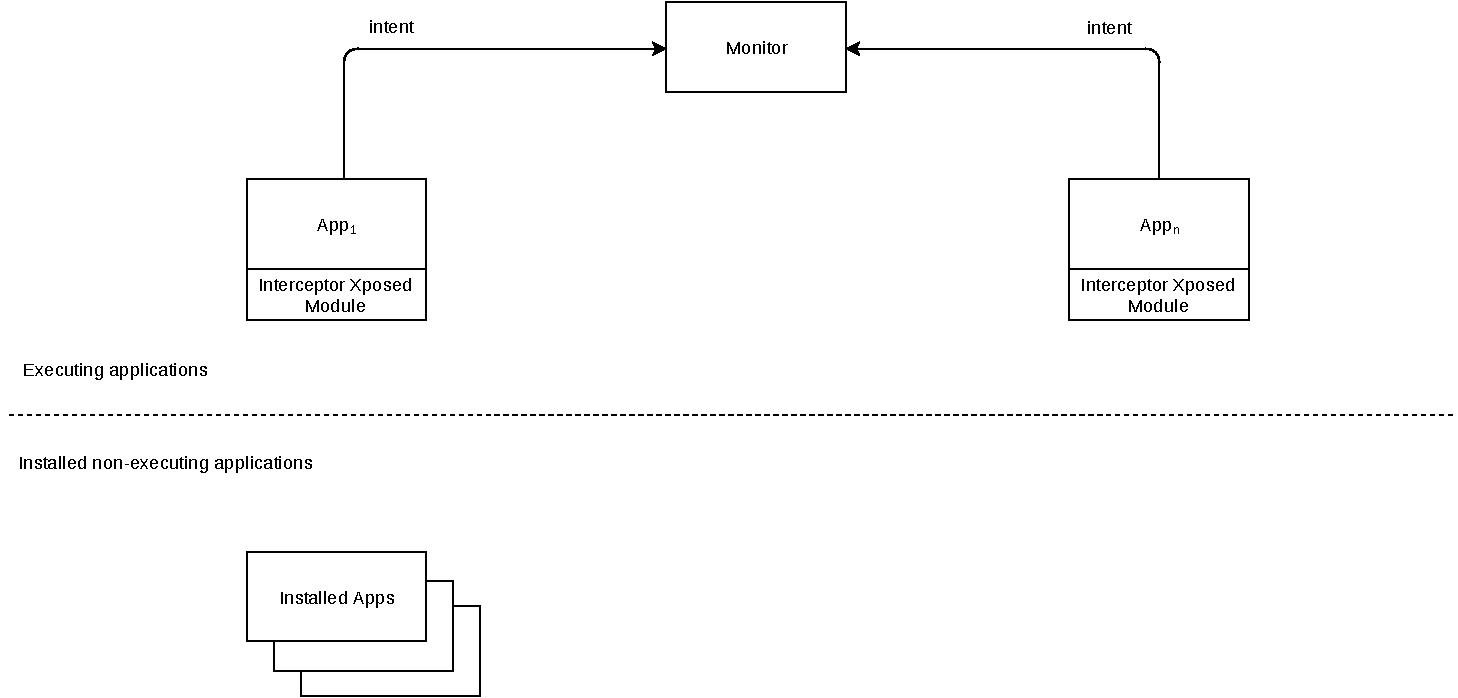
\includegraphics[width=1\textwidth]{graphics/HighLevelArchitecture.pdf}
%\end{center}
%
%For our first attempt to implement a monitor app, we utilised an algorithm by Grigore Ro\c{s}u and Klaus Havelund \cite{RosuHavelund}.  The algorithm appeared interesting thanks to its low complexity: the cost for evaluating a property $\varphi$ on a trace $t$ is $O(|t| * |\varphi|)$, i.e., is linear.  However, the algorithm evaluates a property by traversing the trace from the last event to the first.  This makes it impossible to re-use intermediate results from evaluating $\varphi$ over $t$ for evaluating $\varphi$ over $t {\mathbin{\raise 0.8ex\hbox{$\frown$}}} \langle e \rangle$, i.e., the trace $t$ extended by an event $e$.  In our experiments, this limits the trace length to about 100 events.  Beyond that, the device stopped responding.  Such a trace length is far too short to be of any use in a real-world scenario.
%
%Thus, we created a novel `reverse' version of the algorithm that allows the re-use of intermediate results.  Our new algorithm performs well, i.e., traces can grow to an arbitrary size, and we have tested up to a trace length of 100,000 without encountering any issues.  Evaluation time for new events is in the region of milliseconds for the formula stated above, but this comes at a price: our new algorithm does not support the future LTL operators.
%
%Tests with apps developed for collusion, cf.\ \cite{DetectingMaliciousCollusion}, successfully demonstrated that monitoring is effective on Android hardware without any significant performance reductions.  Evaluation of a new trace event causes CPU usage in the area of 1.5\%.  But to entirely evaluate the performance of our approach, further experimentation into simultaneous monitoring of different security properties will be necessary.  First experiments suggest a linear increase in CPU usage with the total monitored properties.\footnote{Abstract submitted to the CPS-IOT conference for cyber physical systems on the 18th of May 2021 \url{https://sites.google.com/virginia.edu/mt-cps2021/program}}

\end{abstract}
